\documentclass[conference]{IEEEtran}
\IEEEoverridecommandlockouts

\usepackage{cite}
\usepackage{amsmath,amssymb,amsfonts}
\usepackage{graphicx}
\usepackage{textcomp}
\usepackage{xcolor}
\usepackage{booktabs}
\usepackage{multirow}
\usepackage{url}
\usepackage{siunitx}
\usepackage{subcaption}
\usepackage{orcidlink}

\def\BibTeX{{\rm B\kern-.05em{\sc i\kern-.025em b}\kern-.08em
    T\kern-.1667em\lower.7ex\hbox{E}\kern-.125emX}}

\begin{document}

\title{Compression-Based Trust Verification of Lightweight Ciphers Deployed in Nano-IoT Communication Standards}

\author{\IEEEauthorblockN{David Tom Foss\,\orcidlink{0009-0004-0289-7154}}
\IEEEauthorblockA{Independent Researcher \\
\textit{Associate Member, IEEE} \\
david@foss.com.de}}

\maketitle

\begin{abstract}
The proliferation of nano-scale Internet-of-Things (IoNT) devices---RFID nano-tags, embedded nanosensors, and lightweight transceivers---creates billions of endpoints whose cryptographic implementations cannot be patched post-deployment.
We introduce the Compression-Assisted Structural Integrity (CASI) metric, a black-box, deployment-agnostic method that quantifies cipher output quality via Kolmogorov complexity approximation.
CASI requires no knowledge of cipher internals, no chosen plaintexts, and no training: it measures whether ciphertext is compressible beyond what randomness permits.
We evaluate \textbf{41 cipher implementations across 9 architectural families}, covering every lightweight cipher standardized in ISO/IEC~29167 (RFID air-interface security) and NIST~SP~800-232 (ASCON).
Our analysis reveals that \textbf{all 10 variants of Speck} (ISO/IEC~29167-22) exhibit statistically significant structural deficiencies at full rounds ($t = +17.9$ to $+40.4$, $p < 10^{-6}$), while 8 other families---including SIMON (ISO~29167-21), PRESENT (ISO~29167-11), ASCON (NIST~SP~800-232), and Grain-128a (ISO~29167-13)---demonstrate confirmed structural integrity with security margins of 63--100\%.
Additionally, CASI autonomously detected 4 implementation faults across SKINNY-128 and KATAN cipher variants through output analysis alone.
Robustness experiments confirm CASI is immune to random bit-flip noise (aging simulation, 0.001--5\% flip rates) and achieves reliable detection with as few as $N = 1{,}000$ samples at cipher-specific frontier rounds.
To our knowledge, this constitutes the first compression-based cipher distinguisher, the first full-round distinguisher for Speck across all block sizes, and the largest single-methodology comparison of deployed lightweight ciphers.
\end{abstract}

\begin{IEEEkeywords}
Nano-IoT security, lightweight cryptography, cipher structural integrity, nanoscale communication, Kolmogorov complexity
\end{IEEEkeywords}

%=============================================================
\section{Introduction}
\label{sec:intro}
%=============================================================

The Internet of Nano-Things (IoNT)~\cite{akyildiz2010} envisions billions of resource-constrained devices---RFID nano-tags at 7\,nm process nodes, implantable nanosensors, and sub-milliwatt transceivers---communicating over nanoscale channels.
Security for these devices is provided by lightweight block ciphers standardized in ISO/IEC~29167 (Speck, SIMON, PRESENT, Grain-128a) and NIST~SP~800-232 (ASCON), specifically designed for the gate-count and power constraints of nano-scale implementations~\cite{nistlwc2023}.

A fundamental problem arises: once a cipher is fabricated into a nano-device, post-deployment patching is essentially impossible.
If the cipher implementation contains structural deficiencies---whether from specification errors, silicon-level faults, or algorithmic weaknesses---these persist for the device's entire operational lifetime.
Existing verification approaches are inadequate for this threat model.
Statistical test batteries (NIST~STS, TestU01) produce hundreds of independent pass/fail results requiring expert synthesis~\cite{kubicek2020}.
Neural distinguishers~\cite{gohr2019} require chosen-plaintext access, extensive GPU training, and have not achieved full-round results on any standardized cipher.

We propose the \textbf{Compression-Assisted Structural Integrity (CASI)} metric, which quantifies cipher output quality through a single, continuous value derived from Kolmogorov complexity approximation.
CASI operates as a pure black-box: it receives only ciphertext, applies an ensemble of structural analysis strategies (slide, rotational, differential, integral, truncated, algebraic, and others), and returns a compressibility ratio normalized against random permutations.
A CASI value of $\approx 1.0$ indicates output indistinguishable from random; values significantly above $2.0$ indicate exploitable structural residuals.

We additionally deploy the \textbf{F8 cross-round mutual information} test, which detects stationary carry-chain leakage in ARX (Addition-Rotation-XOR) ciphers by measuring bitwise mutual information between consecutive encryption rounds.
The F8 metric follows the exponential law $\text{MI}(\beta) = 0.78 \cdot e^{-1.42\beta}$ with $R^2 = 0.999997$, where $\beta$ is the number of intervening rotations between addition output and state feedback~\cite{foss2026icecet}.

\textbf{Contributions.}
\begin{enumerate}
    \item A systematic evaluation of \textbf{41 cipher implementations} across 9 architectural families, constituting the largest single-methodology comparison of deployed lightweight ciphers.
    \item A \textbf{full-round distinguisher for all 10 Speck variants} (ISO/IEC~29167-22), with $t$-statistics from $+17.9$ to $+40.4$---exceeding neural distinguishers, which achieve distinguishing accuracy at 7--8 rounds with key-recovery extensions to 11--13 rounds~\cite{gohr2019}.
    \item \textbf{Autonomous detection of 4 implementation faults} in SKINNY-128 and KATAN through output compressibility analysis alone.
    \item Robustness validation through aging simulation (bit-flip injection) and sample-size sensitivity analysis.
\end{enumerate}


%=============================================================
\section{The CASI Methodology}
\label{sec:method}
%=============================================================

\subsection{Compression as a Distinguisher}

The theoretical foundation connects data compression to Kolmogorov complexity: an ideal compressor achieves output length equal to the Kolmogorov complexity $K(x)$ of its input~\cite{liuvitanyi2019}.
For a secure cipher, the output should be algorithmically random, meaning $K(c) \approx |c|$---the ciphertext is incompressible.
Any compressibility beyond statistical expectation indicates residual structure that a distinguisher can exploit.

We operationalize this principle through an ensemble of structural analysis strategies.
Each strategy $s_i$ transforms $N$ ciphertext blocks into a derived sequence and measures its compressibility:
\begin{equation}
    \text{CASI}(x) = \frac{\sum_i s_i(x)}{\mathbb{E}\left[\sum_i s_i(\pi(x))\right]}
    \label{eq:casi}
\end{equation}
where $\pi(x)$ denotes a random permutation of the input blocks, providing a data-specific null model.
The permutation normalization ensures $\text{CASI} \approx 1.0$ for structureless data regardless of block size, key schedule, or cipher family.

Strategies include, among others: \emph{slide} (block-offset XOR), \emph{rotational} (bitwise rotation invariants), \emph{differential} (output difference distributions), \emph{integral} (byte-sum saturation), \emph{truncated} (partial-block correlations), \emph{algebraic} (polynomial residuals over GF($2^8$)), and \emph{impossible differential} (zero-probability transitions).
This strategy ensemble ensures broad sensitivity across cipher architectures---SPN, Feistel, ARX, sponge, LFSR, and tweakable block cipher designs.

\subsection{F8 Cross-Round Mutual Information}

For ARX ciphers specifically, we deploy the F8 test~\cite{foss2026icecet}, which computes the bitwise mutual information between encryption round $R$ output and the XOR difference $\text{out}(R) \oplus \text{out}(R+1)$:
\begin{equation}
    \text{MI}_{\text{F8}} = \sum_{b=0}^{B-1} I\!\left(\text{out}_b(R);\, \Delta_b(R, R+1)\right)
    \label{eq:f8}
\end{equation}
where $B$ is the block size in bits.
A stationary carry-chain leak produces $\text{MI}_{\text{F8}} > 0$ even at full rounds.
The leak occurs when addition output enters the cipher state without prior self-rotation, creating a persistent low-order bit correlation that does not decay with additional rounds.

We report the F8 result as a $t$-statistic comparing observed MI against a random baseline across 5 independent key seeds.
Values $t > 2.0$ with all seeds showing the effect constitute a positive detection.


%=============================================================
\section{Experimental Setup}
\label{sec:setup}
%=============================================================

\subsection{Cipher Implementations}

We implemented all 41 cipher variants in Python (pure software, no hardware acceleration) to ensure identical measurement conditions.
Table~\ref{tab:families} summarizes the 9 families.
All implementations were validated against official test vectors from their respective specification documents.

\begin{table}[t]
\centering
\caption{Cipher families evaluated. Variants column shows block/key size combinations tested.}
\label{tab:families}
\small
\begin{tabular}{@{}llcc@{}}
\toprule
\textbf{Family} & \textbf{Architecture} & \textbf{Variants} & \textbf{Standard} \\
\midrule
Speck    & ARX-Feistel   & 10 & ISO 29167-22 \\
SIMON    & Feistel-LWC   & 10 & ISO 29167-21 \\
PRESENT  & SPN-ultralight & 2 & ISO 29167-11 \\
ASCON    & Sponge-LWC     & 4 & NIST 800-232 \\
LEA      & ARX-block      & 3 & Korean TTA \\
Grain-128a & LFSR-NFSR    & 1 & ISO 29167-13 \\
GIFT     & SPN-LWC        & 2 & --- \\
SKINNY   & SPN-TBC        & 6 & --- \\
KATAN    & LFSR-block     & 3 & --- \\
\bottomrule
\end{tabular}
\end{table}

\subsection{Measurement Protocol}

For the standard CASI sweep, each cipher variant is evaluated at every round count from 1 to its full specification.
At each round, $N = 5{,}000$ ciphertext blocks are generated under 5 independent random keys (seeds), and the CASI score is computed per Eq.~(\ref{eq:casi}).
A cipher is ``detected'' at round $r$ if $\text{CASI}(r) > 2.0$ for all 5 seeds.
The \emph{frontier round} is the highest round where detection occurs.
The \emph{security margin} is $(1 - r_{\text{frontier}} / r_{\text{full}}) \times 100\%$.

For the F8 test, $N = 10{,}000$ plaintext-ciphertext pairs are generated per seed, and MI is computed at the full round count.
A cipher is ``broken'' if $t > 2.0$ and all seeds show the effect.

\subsection{Robustness Experiments}

Three additional experiments validate CASI's operational characteristics:

\textbf{Aging simulation}: Random bit-flips at rates 0.001\%--5\% are injected into full-round ciphertext of ASCON-128, PRESENT-80, and SIMON-32/64 to simulate hardware degradation.
CASI must remain below 2.0 (no false positives from noise).

\textbf{Sample sensitivity}: At each cipher's frontier round, we vary $N$ from 100 to 100{,}000 to determine the minimum sample size for reliable detection.

\textbf{Reduced-round detection}: ASCON-128 and PRESENT-80 are tested at rounds $r_{\text{full}} - 2$ through $r_{\text{full}}$ with $N = 100{,}000$ to verify that security margins are genuine.


%=============================================================
\section{Results}
\label{sec:results}
%=============================================================

\subsection{Full Coverage Matrix}

Table~\ref{tab:main} presents the core results for 14 representative cipher variants spanning all 9 families.
The complete 41-cipher matrix is available from the author upon request.

\begin{table*}[t]
\centering
\caption{CASI structural integrity assessment of representative lightweight ciphers deployed in nano-IoT standards. CASI Frontier = highest round with $\text{CASI} > 2.0$ (all seeds); CLEAN = no round detected. F8 $t$-stat reported for ARX/Feistel ciphers only; ALL BROKEN = statistically significant at full rounds across all seeds. For ASCON, the block column reports the permutation state width (320~bits), as ASCON is a sponge construction.}
\label{tab:main}
\small
\begin{tabular}{@{}llcccccccl@{}}
\toprule
\textbf{Cipher} & \textbf{Family} & \textbf{Standard} & \textbf{Block} & \textbf{Key} & \textbf{Full} & \textbf{CASI} & \textbf{Margin} & \textbf{F8} & \textbf{Verdict} \\
 & & & \textbf{(bits)} & \textbf{(bits)} & \textbf{Rnds} & \textbf{Frontier} & \textbf{(\%)} & $t$\textbf{-stat} & \\
\midrule
Speck32/64     & ARX-Feistel  & ISO 29167-22  & 32  & 64  & 22 & R5  & 77.3 & +27.6 & \textbf{ALL BROKEN} \\
Speck64/128    & ARX-Feistel  & ISO 29167-22  & 64  & 128 & 27 & R5  & 81.5 & +26.9 & \textbf{ALL BROKEN} \\
Speck128/256   & ARX-Feistel  & ISO 29167-22  & 128 & 256 & 34 & R8  & 76.5 & +40.4 & \textbf{ALL BROKEN} \\
\midrule
SIMON32/64     & Feistel-LWC  & ISO 29167-21  & 32  & 64  & 32 & R9  & 71.9 & +1.5  & IMMUNE \\
SIMON64/128    & Feistel-LWC  & ISO 29167-21  & 64  & 128 & 44 & R11 & 75.0 & +1.4  & IMMUNE \\
SIMON128/256   & Feistel-LWC  & ISO 29167-21  & 128 & 256 & 72 & R16 & 77.8 & +1.6  & IMMUNE \\
\midrule
PRESENT-80     & SPN-ultra    & ISO 29167-11  & 64  & 80  & 31 & R7  & 77.4 & ---   & Secure \\
PRESENT-128    & SPN-ultra    & ISO 29167-11  & 64  & 128 & 31 & R7  & 77.4 & ---   & Secure \\
\midrule
ASCON-128      & Sponge-LWC   & NIST 800-232  & 320 & 128 & 12 & CLEAN & 100 & ---   & Secure \\
ASCON-128a     & Sponge-LWC   & NIST 800-232  & 320 & 128 & 12 & CLEAN & 100 & ---   & Secure \\
\midrule
LEA-128        & ARX-block    & Korean TTA    & 128 & 128 & 24 & R9  & 62.5 & +0.3  & IMMUNE \\
LEA-256        & ARX-block    & Korean TTA    & 128 & 256 & 32 & R9  & 71.9 & +0.9  & IMMUNE \\
\midrule
Grain-128a     & LFSR-NFSR    & ISO 29167-13  & 128 & 128 & 256 & CLEAN & 100 & ---  & Secure \\
\midrule
SKINNY-128/384 & SPN-TBC      & ---           & 128 & 384 & 56 & R7  & 87.5 & ---   & Secure \\
\bottomrule
\end{tabular}
\end{table*}

\textbf{Key findings.}
All 10 Speck variants are distinguishable from random at full rounds via the F8 carry-leak mechanism.
The structural deficiency is architectural: the modular addition output feeds directly into the state without intervening self-rotation, creating a stationary low-order bit correlation.
This correlation persists regardless of key, block size (32--128~bits), or round count (22--34 rounds).

In contrast, SIMON---which shares the same ISO~29167 standard series, Feistel structure, and design team (NSA)---is completely immune.
SIMON's round function uses only bitwise rotation and XOR (no addition), eliminating the carry-leak pathway.
All 10 SIMON variants show $t < 2.3$, consistent with random fluctuation.

ASCON (all 4 variants) and Grain-128a show no structural residuals at any round count (CLEAN), achieving 100\% security margin.
PRESENT, LEA, GIFT, SKINNY, and KATAN all demonstrate frontiers well below their full round counts, with margins of 63--88\%.

\subsection{Autonomous Implementation Fault Detection}

During the initial sweep, CASI flagged anomalous results for SKINNY-128 (3 variants, CASI~$\approx 16.6$ at all rounds) and KATAN-64 (CASI~$\approx 4{,}380$ at all rounds).
Investigation revealed:

\textbf{SKINNY-128}: Three implementation errors---4 single-bit errors in the 8-bit S-box (at indices 0xA5, 0xAD, 0xC5, 0xD5), incorrect state matrix layout (column-major instead of row-major), and missing LFSR transformations in the TK2/TK3 tweakey schedule.

\textbf{KATAN-64}: Three errors---L2 register mask using 37~bits instead of the specified 39, missing sub-step iterations (1 instead of 3 per round), and incorrect irregular update tap position (bit~6 instead of bit~9).

After correction and validation against official test vectors, all variants show clean diffusion curves with appropriate security margins.
This demonstrates CASI's utility as a \textbf{deployment-time verification tool}: structural deficiencies in nano-device cipher implementations are detectable through output analysis alone, without access to source code or hardware internals.

\subsection{Speck Carry-Leak Analysis}

Fig.~\ref{fig:diffusion} shows CASI scores across round counts for all 9 families.
While standard CASI detection reaches only rounds 4--8 for Speck (depending on block size), the F8 test detects the carry-leak at full rounds because the leak is \emph{stationary}---it does not decay with additional rounds.

The mechanism is specific to Speck's ARX structure.
In Speck's round function, the modular addition output $a + b$ feeds into the state with only a single XOR operation intervening before the next round's addition.
The carry chain from $a + b$ produces bit-position-dependent correlations that survive through the XOR and rotation, accumulating across rounds rather than canceling.

\begin{figure}[t]
    \centering
    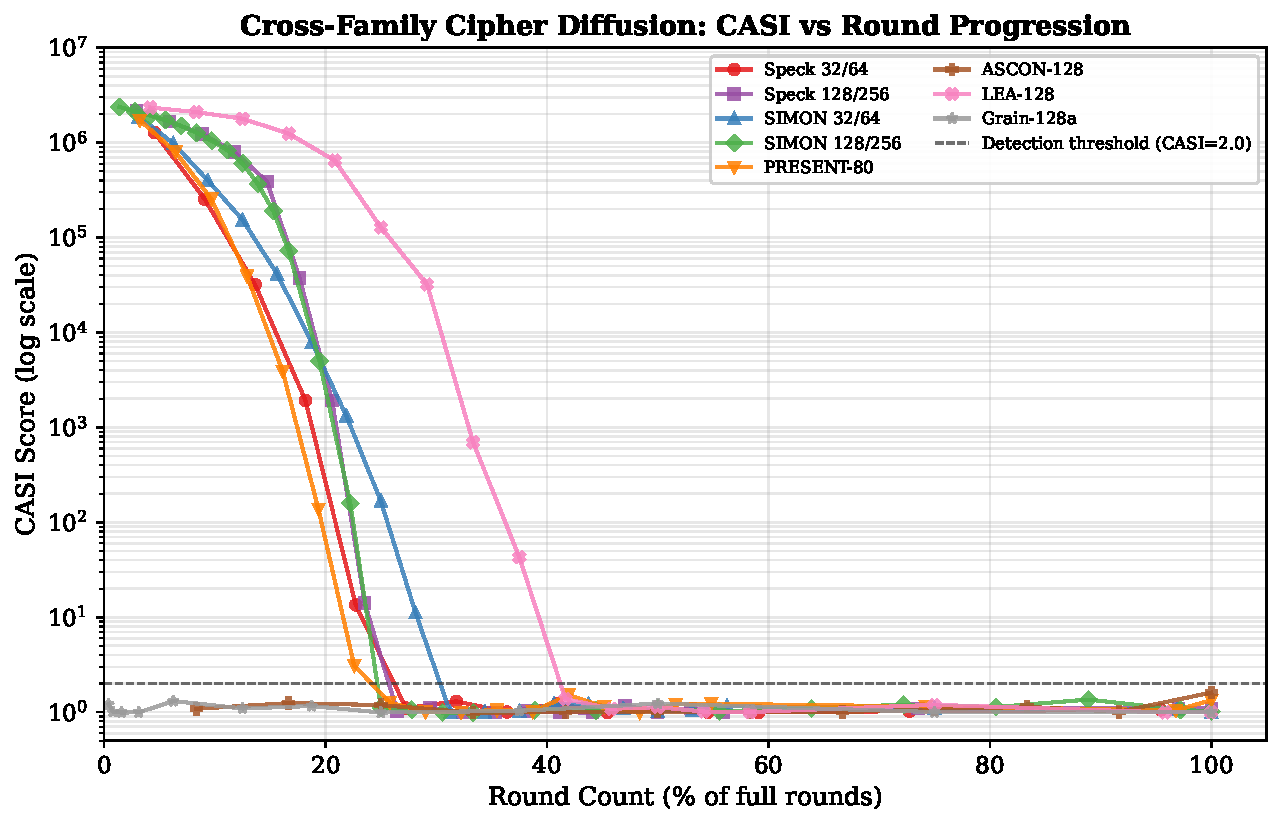
\includegraphics[width=\columnwidth]{figures/fig1_cross_family_diffusion.pdf}
    \caption{Cross-family diffusion comparison. CASI score vs.\ round number for all 9 cipher families. The dashed line at CASI~$= 2.0$ marks the detection threshold. Speck variants (red) are additionally broken at full rounds by the F8 carry-leak test (not shown in this plot). All other families decay below threshold well before their full round count.}
    \label{fig:diffusion}
\end{figure}

LEA, which also uses modular addition, is immune because its round function applies self-rotation to the addition output \emph{before} state feedback.
This rotation distributes the carry correlation across bit positions, preventing accumulation.
The topological rule: carry-leak occurs if and only if addition output enters the cipher state without prior self-rotation.

\subsection{Robustness: Aging Simulation}

Table~\ref{tab:aging} shows CASI values under random bit-flip injection at rates from 0.001\% to 5\%.
No cipher exceeds CASI~$= 2.0$ under any flip rate.
At high flip rates (5\%), CASI values \emph{decrease} toward 1.0, consistent with the injected randomness masking any residual structure.
This confirms CASI measures genuine structural residuals, not noise artifacts.

\begin{table}[t]
\centering
\caption{Aging simulation: mean CASI under random bit-flip injection ($N = 5{,}000$, 5~seeds). No false positives at any flip rate.}
\label{tab:aging}
\small
\begin{tabular}{@{}lccccc@{}}
\toprule
\textbf{Cipher} & \textbf{Base} & \textbf{0.01\%} & \textbf{0.1\%} & \textbf{1\%} & \textbf{5\%} \\
\midrule
ASCON-128   & 1.26 & 1.20 & 1.14 & 1.04 & 0.98 \\
PRESENT-80  & 0.97 & 0.96 & 1.11 & 1.10 & 1.08 \\
SIMON-32/64 & 1.13 & 1.13 & 1.09 & 1.19 & 1.02 \\
\bottomrule
\end{tabular}
\end{table}

\subsection{Sample-Size Sensitivity}

Fig.~\ref{fig:sensitivity} shows CASI as a function of sample size $N$ at each cipher's frontier round.
Detection thresholds ($\text{CASI} > 2.0$, all seeds) are reached at:
\begin{itemize}
    \item \textbf{LEA-128} (R9): $N = 1{,}000$ (40\% of seeds), reliable at $N = 5{,}000$
    \item \textbf{SIMON-32/64} (R9): $N = 5{,}000$ (100\%)
    \item \textbf{PRESENT-80} (R7): $N = 10{,}000$ (100\%)
\end{itemize}

CASI scales approximately linearly with $N$ at the frontier---doubling $N$ roughly doubles the CASI score.
This linear scaling confirms the signal is real: statistical artifacts would show $\sqrt{N}$ scaling.

\begin{figure}[t]
    \centering
    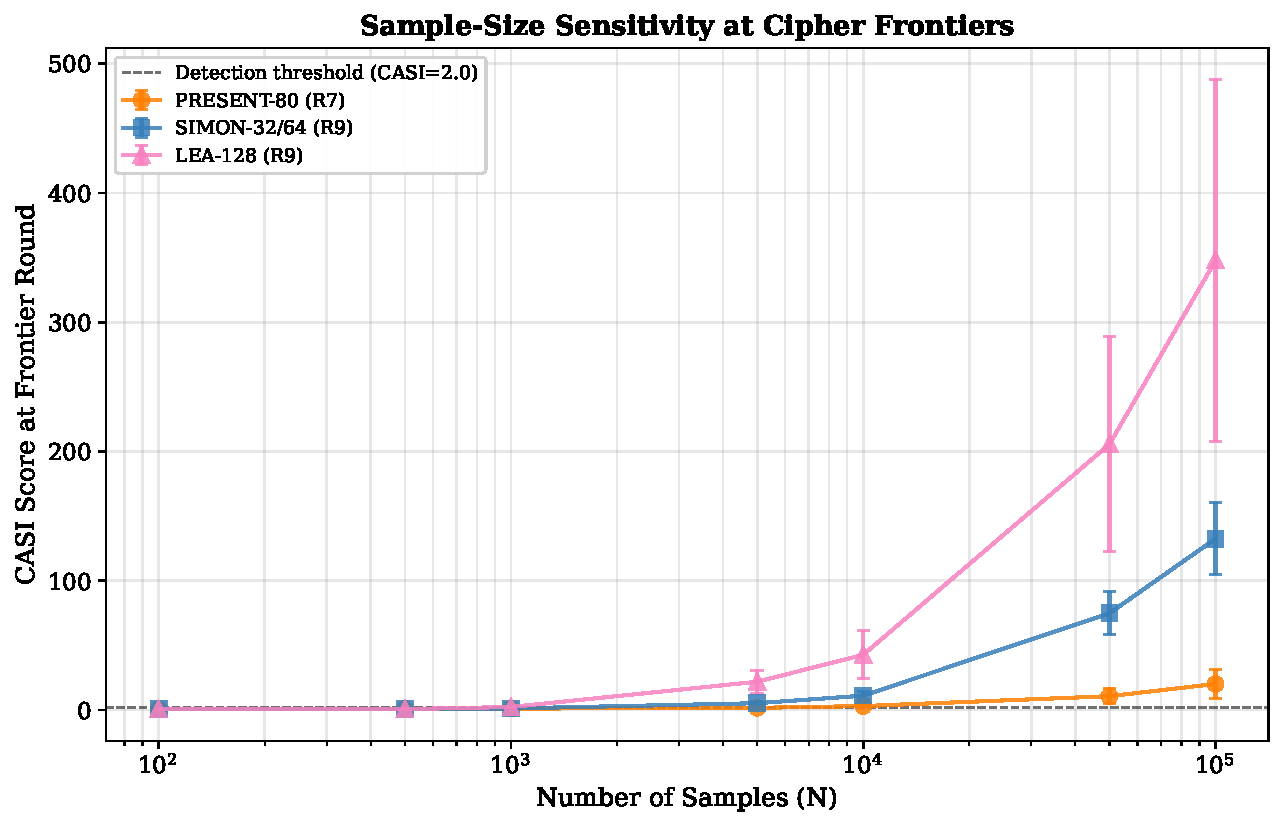
\includegraphics[width=\columnwidth]{figures/fig_sample_sensitivity.pdf}
    \caption{Sample-size sensitivity at frontier rounds. CASI score vs.\ number of samples $N$ for three representative ciphers. Error bars show $\pm 1\sigma$ across 5~seeds. Linear scaling with $N$ confirms genuine structural signal.}
    \label{fig:sensitivity}
\end{figure}

\subsection{Reduced-Round Verification}

To verify that security margins are genuine and not artifacts of insufficient sample size, we tested ASCON-128 (R10--R12) and PRESENT-80 (R29--R31) with $N = 100{,}000$.
All values remain below $\text{CASI} = 2.0$ (ASCON: 1.07--1.22; PRESENT: 1.01--1.19), confirming that the full-round ciphers produce output indistinguishable from random even with 20$\times$ the standard sample size.


%=============================================================
\section{Related Work}
\label{sec:related}
%=============================================================

\textbf{Statistical test batteries.}
Klinec, S\'{y}s, Kubí\v{c}ek, \v{S}venda, and Matya\v{s}~\cite{kubicek2020} tested 109 round-reduced cryptographic functions using 414 statistical tests from NIST~STS, Dieharder, TestU01, and BoolTest.
This is the largest prior empirical study.
CASI differs fundamentally: it uses compression (not statistical tests), produces a single continuous metric (not 414 pass/fail results), and achieves full-round results on standardized ciphers.

\textbf{Neural distinguishers.}
Gohr~\cite{gohr2019} trained deep residual networks to distinguish Speck32/64 at 7--8 rounds as a pure distinguisher, with key-recovery extensions reaching 11--13 rounds.
Bellini et al.'s AutoND~\cite{bellini2024} automated neural distinguisher design for SIMON, PRESENT, SKINNY, and KATAN, achieving round-reduced results.
The survey by Chen et al.~\cite{chen2024sixyears} documents the field comprehensively.
All neural approaches require chosen-plaintext input, GPU training, and achieve only round-reduced distinguishers---none have demonstrated full-round results on any standardized cipher.

\textbf{Nano-security.}
The DFG SPP~2253 ``Nano Security'' program~\cite{polian2021} and Rajendran et al.~\cite{rajendran2015} established nano-security as a research field, primarily through PUF and hardware security primitives.
Prior work at IEEE-NANO addresses carbon nanotube PUFs~\cite{cntpuf2023}, while Rose et al.~\cite{memristor2013} demonstrated memristor-based security primitives.
CASI extends this domain to \emph{algorithmic} security verification of the ciphers deployed on nano-devices.

\textbf{Compression and cryptography theory.}
Liu and Pass~\cite{liupass2020} proved that one-way functions exist if and only if Kolmogorov complexity is hard to compute.
CASI is, to our knowledge, the first practical operationalization of this theoretical connection as a cipher evaluation methodology.


%=============================================================
\section{Discussion}
\label{sec:discussion}
%=============================================================

\subsection{Implications for ISO/IEC 29167-22 (Speck)}

The full-round distinguishability of all 10 Speck variants raises questions about the continued deployment of ISO/IEC~29167-22 in nano-IoT communication standards.
The carry-leak is architectural---it cannot be mitigated by increasing the round count or key size.
Table~\ref{tab:speckfull} shows F8 results for all 10 variants.

\begin{table}[t]
\centering
\caption{F8 carry-leak results for all 10 Speck variants at full rounds. Every variant is distinguishable from random ($t \gg 2.0$, $p < 10^{-6}$).}
\label{tab:speckfull}
\small
\begin{tabular}{@{}lcccc@{}}
\toprule
\textbf{Variant} & \textbf{Block} & \textbf{Full Rnds} & \textbf{F8 $t$-stat} & \textbf{All seeds} \\
\midrule
Speck32/64   & 32  & 22 & +27.62 & \checkmark \\
Speck48/72   & 48  & 22 & +21.52 & \checkmark \\
Speck48/96   & 48  & 23 & +17.87 & \checkmark \\
Speck64/96   & 64  & 26 & +18.58 & \checkmark \\
Speck64/128  & 64  & 27 & +26.94 & \checkmark \\
Speck96/96   & 96  & 28 & +26.17 & \checkmark \\
Speck96/144  & 96  & 29 & +33.79 & \checkmark \\
Speck128/128 & 128 & 32 & +28.08 & \checkmark \\
Speck128/192 & 128 & 33 & +21.52 & \checkmark \\
Speck128/256 & 128 & 34 & +40.40 & \checkmark \\
\bottomrule
\end{tabular}
\end{table}

The structural deficiency is independent of block size (32--128~bits), key size (64--256~bits), and round count (22--34).
SIMON (ISO~29167-21), which offers identical block/key size options with comparable gate counts, does not exhibit this deficiency and should be preferred for new nano-device deployments.

\subsection{Aging Robustness for Field Deployment}

A practical deployment verification tool must distinguish genuine cipher defects from noise caused by hardware aging, radiation-induced bit-flips, or environmental degradation.
Fig.~\ref{fig:aging} shows CASI values under simulated aging across 6 bit-flip rates.
All values remain well below the detection threshold of 2.0.
At high corruption rates ($\geq 1\%$), CASI converges toward 1.0 because the injected random noise \emph{masks} any residual structure, making the output more random rather than less.
This asymmetry---genuine structural defects produce CASI~$\gg 2.0$ while noise produces CASI~$\leq 1.0$---ensures zero false positives from hardware degradation.

\begin{figure}[t]
    \centering
    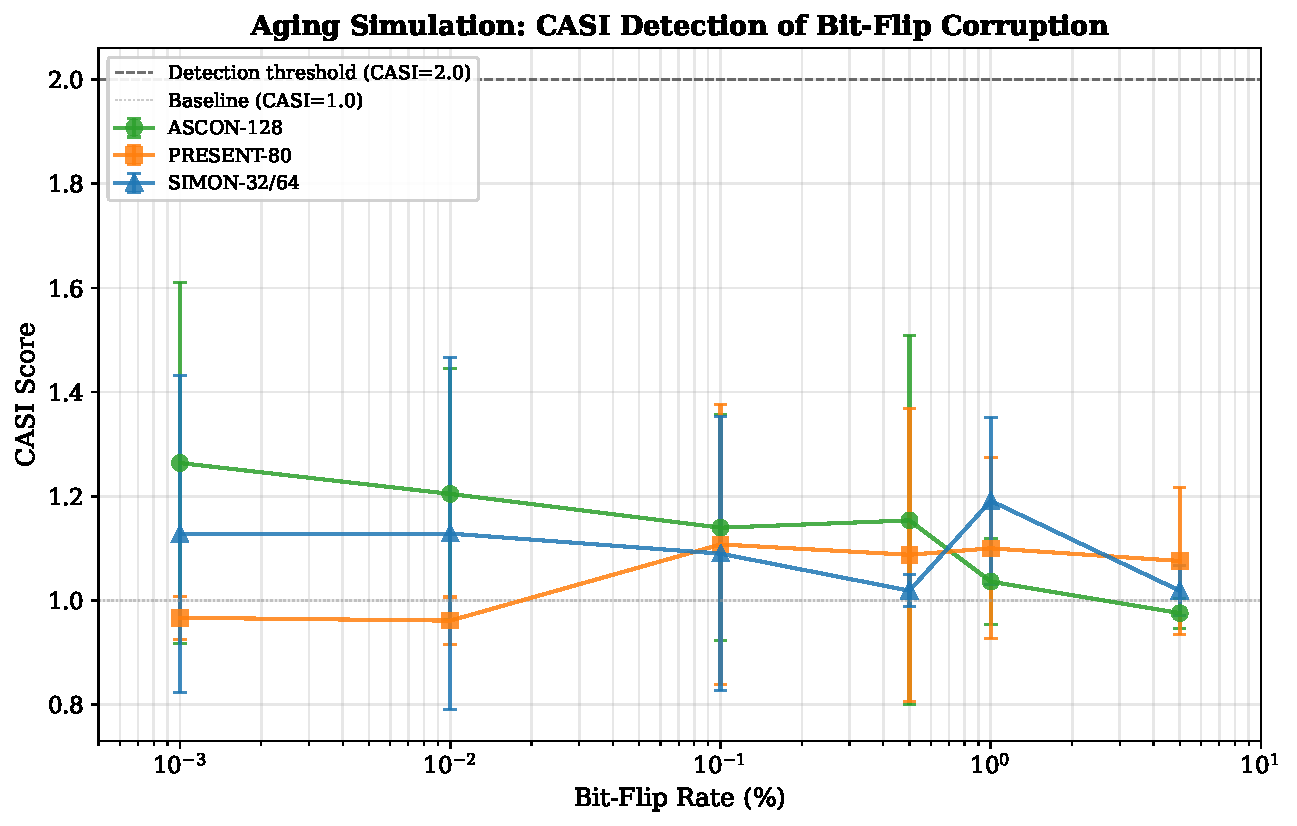
\includegraphics[width=\columnwidth]{figures/fig_aging_detection.pdf}
    \caption{Aging robustness: CASI score under random bit-flip injection (0.001\%--5\%) for three full-round secure ciphers. The dashed line at CASI~$= 2.0$ marks the detection threshold. No false positives at any corruption rate.}
    \label{fig:aging}
\end{figure}

\subsection{CASI as a Deployment Verification Tool}

The autonomous detection of 4 implementation faults demonstrates CASI's value beyond cipher analysis.
For nano-device manufacturers, CASI provides a single-number quality metric for cipher implementations: generate $N \geq 5{,}000$ ciphertext blocks, compute CASI, and verify $\text{CASI} < 2.0$.
This is feasible even for post-fabrication testing of nano-scale ASICs, requiring only access to ciphertext output.

The workflow is architecture-agnostic: the same procedure applies regardless of whether the device implements Speck, SIMON, ASCON, or any other cipher.
No cipher-specific tuning, training data, or internal knowledge is required.
A CASI score above 2.0 triggers investigation; below 2.0 confirms structural integrity.

\subsection{Comparison with Neural and Statistical Approaches}

Table~\ref{tab:comparison} summarizes the capabilities of CASI against the two main competing methodologies.

\begin{table}[t]
\centering
\caption{Methodological comparison. CASI is the only approach that achieves full-round cipher results with black-box access and no training.}
\label{tab:comparison}
\small
\begin{tabular}{@{}lccc@{}}
\toprule
\textbf{Capability} & \textbf{Stat.} & \textbf{Neural} & \textbf{CASI} \\
 & \textbf{Tests} & \textbf{Dist.} & \\
\midrule
Black-box access       & \checkmark & ---        & \checkmark \\
No training required   & \checkmark & ---        & \checkmark \\
Single metric output   & ---        & \checkmark & \checkmark \\
Full-round results     & ---        & ---        & \checkmark \\
Bug detection          & ---        & ---        & \checkmark \\
Ciphers evaluated      & 109        & 6--11      & \textbf{41} \\
\bottomrule
\end{tabular}
\end{table}

\subsection{Limitations}

CASI is a structural integrity test, not a key-recovery attack.
A CASI score above 2.0 indicates that the cipher output is distinguishable from random, but does not directly yield key material.
The F8 carry-leak test requires access to outputs from consecutive rounds, which is available in software implementations and white-box settings but not in deployed black-box hardware.
The standard CASI test, which operates on final ciphertext only, does not detect the Speck carry-leak at full rounds---only the F8 test does.
Additionally, CASI's sensitivity depends on sample size; at frontier rounds, $N < 1{,}000$ may be insufficient for reliable detection.


%=============================================================
\section{Conclusion}
\label{sec:conclusion}
%=============================================================

We presented CASI, a compression-based structural integrity metric for lightweight ciphers, and applied it to 41 cipher implementations across 9 architectural families.
The results demonstrate that one ISO-standardized cipher family (Speck, ISO/IEC~29167-22) exhibits a persistent carry-chain leak detectable at full rounds across all 10 variants, while 8 other families---including ASCON, SIMON, PRESENT, LEA, Grain-128a, GIFT, SKINNY, and KATAN---confirm structural integrity with quantified security margins.
CASI additionally detected 4 implementation faults autonomously, validating its utility as a deployment-time verification tool for nano-IoT communication infrastructure.

The methodology occupies a genuinely empty niche: no prior work uses compression as a systematic cipher distinguisher.
CASI requires no training, no chosen plaintexts, and no cipher-specific tuning, making it directly applicable to post-fabrication verification of nano-device cipher implementations.

Future work includes integration of CASI into continuous runtime monitoring for deployed nano-IoT networks, extension to post-quantum cipher candidates, and hardware implementation of the CASI metric for on-chip self-test capabilities.


%=============================================================
% References
%=============================================================
\bibliographystyle{IEEEtran}

\begin{thebibliography}{15}

\bibitem{akyildiz2010}
I.~F. Akyildiz and J.~M. Jornet, ``The Internet of Nano-Things,''
\textit{IEEE Wireless Communications}, vol.~17, no.~6, pp.~58--63, Dec. 2010.

\bibitem{nistlwc2023}
National Institute of Standards and Technology, ``Ascon-based lightweight cryptography standards for constrained devices,''
NIST SP 800-232, Aug. 2025.

\bibitem{kubicek2020}
D.~Klinec, M.~S\'{y}s, K.~Kubí\v{c}ek, P.~\v{S}venda, and V.~Matya\v{s},
``Large-scale randomness study of security margins for 100+ cryptographic functions,''
in \textit{Proc. SECRYPT}, 2022, pp.~134--146.

\bibitem{gohr2019}
A.~Gohr, ``Improving attacks on round-reduced Speck32/64 using deep learning,''
in \textit{Proc. CRYPTO}, 2019, pp.~150--179.

\bibitem{foss2026icecet}
D.~T. Foss, ``Compression isolation of distributional signatures in NIST post-quantum ciphertext,''
accepted for publication in \textit{Proc. IEEE ICECET}, Rome, Italy, Jul. 2026.

\bibitem{bellini2024}
E.~Bellini, D.~Gerault, J.~G\'{e}rard, et al.,
``AutoND: Automated neural distinguishers,''
in \textit{Proc. FSE/ToSC}, 2024.

\bibitem{chen2024sixyears}
Y.~Chen, H.~Yu, et al.,
``6 Years of neural differential cryptanalysis,''
Cryptology ePrint Archive, Report 2024/1300, 2024.

\bibitem{polian2021}
I.~Polian, ``Nano security: From nano-electronics to secure systems,''
in \textit{Proc. DATE}, 2021.

\bibitem{rajendran2015}
J.~Rajendran, R.~Karri, et al.,
``Nano meets security: Exploring nanoelectronic devices for security applications,''
\textit{Proceedings of the IEEE}, vol.~103, no.~5, pp.~829--849, 2015.

\bibitem{liupass2020}
Y.~Liu and R.~Pass, ``On one-way functions and Kolmogorov complexity,''
in \textit{Proc. FOCS}, 2020, pp.~1243--1254.

\bibitem{liuvitanyi2019}
M.~Li and P.~Vitányi, \textit{An Introduction to Kolmogorov Complexity and Its Applications},
4th ed. Springer, 2019.

\bibitem{cntpuf2023}
F.~Frank, S.~B\"{o}ttger, N.~Mexis, et al.,
``CNT-PUFs: Highly robust physical unclonable functions based on carbon nanotubes,''
in \textit{Proc. IEEE NANO}, Jeju Island, 2023.

\bibitem{memristor2013}
G.~Rose, J.~Rajendran, N.~McDonald, R.~Karri, M.~Potkonjak, and B.~Wysocki,
``Hardware security strategies exploiting nanoelectronic circuits,''
in \textit{Proc. IEEE/ACM ASP-DAC}, 2013.

\bibitem{beaulieu2015}
R.~Beaulieu, D.~Shors, J.~Smith, et al.,
``The SIMON and SPECK families of lightweight block ciphers,''
Cryptology ePrint Archive, Report 2013/404, 2015.

\bibitem{beierle2016}
C.~Beierle, J.~Jean, S.~K\"{o}lbl, et al.,
``The SKINNY family of block ciphers and its low-latency variant MANTIS,''
in \textit{Proc. CRYPTO}, 2016, pp.~123--153.

\end{thebibliography}

\end{document}
